% Intended LaTeX compiler: pdflatex
\documentclass[11pt]{article}
\usepackage[utf8]{inputenc}
\usepackage[T1]{fontenc}
\usepackage{graphicx}
\usepackage{longtable}
\usepackage{wrapfig}
\usepackage{rotating}
\usepackage[normalem]{ulem}
\usepackage{amsmath}
\usepackage{amssymb}
\usepackage{capt-of}
\usepackage{hyperref}
\author{Construção de compiladores I}
\date{}
\title{Semântica de IMP}
\hypersetup{
 pdfauthor={Construção de compiladores I},
 pdftitle={Semântica de IMP},
 pdfkeywords={},
 pdfsubject={},
 pdfcreator={Emacs 28.2 (Org mode 9.7)}, 
 pdflang={English}}
\begin{document}

\maketitle
\section*{Objetivos}
\label{sec:org05319c8}

\subsection*{Objetivos}
\label{sec:orgaf7b2c4}

\begin{itemize}
\item Apresentar a semântica operacional para a linguagem IMP.

\item Implementar um interpretador de IMP.
\end{itemize}
\section*{Introdução}
\label{sec:orgd5ca1f4}

\subsection*{Introdução}
\label{sec:org5d4e26a}

\begin{itemize}
\item Na última aula, apresentamos uma semântica operacional para uma linguagem de expressões.

\item Implementamos um interpretador a partir da semântica desta linguagem.
\end{itemize}
\subsection*{Introdução}
\label{sec:org831e662}

\begin{itemize}
\item Porém, o que vimos não é suficiente para lidar com linguagens imperativas.

\item Como lidar com a manipulação de variáveis?
\end{itemize}
\subsection*{Introdução}
\label{sec:org23b1ac9}

\begin{itemize}
\item Para lidar com variáveis, vamos adicionar uma abstração para representar a memória.
\end{itemize}
\section*{Sintaxe de Imp}
\label{sec:orgbd0e277}

\subsection*{Sintaxe de Imp}
\label{sec:org050a016}

\begin{itemize}
\item Recapitulando: Sintaxe de Imp
\end{itemize}

\begin{array}{lcl}
Program   & \to  & Stmts\\
Stmts     & \to & Statement\:\:Stmts\,\mid\,\lambda\\
\end{array}
\subsection*{Sintaxe de Imp}
\label{sec:org17d4805}

\begin{itemize}
\item Recapitulando: Sintaxe de Imp
\end{itemize}

\begin{array}{lcl}
Statement & \to  & \mathtt{skip ;}\:\:\mid\:\:Type\:\:\mathrm{id}\:\:Init \mathrm{;} \\
          & \mid & \mathrm{id}\:\:\mathtt{:=}\:\:Expr\mathrm{;}\\
          & \mid & \mathtt{read}\:\:\mathrm{id ;}\:\:\mid\:\:\mathtt{print}\:\:Expr \mathrm{;}\\
          & \mid & \mathtt{if}\:\:Expr\:\:\mathtt{then}\:\:Block\\
          & \mid & \mathtt{if}\:\:Expr\:\:\mathtt{then}\:\:Block\:\:\mathrm{else}\:\:Block\\
          & \mid & \mathtt{while}\:\:Expr\:\:Block
\end{array}
\subsection*{Sintaxe de Imp}
\label{sec:orga6ec68a}

\begin{itemize}
\item Recapitulando: Sintaxe de Imp
\end{itemize}

\begin{array}{lcl}
Expr & \to  & Expr\:\:Op\:\:Expr\\
     & \mid & \mathrm{-}\:\: Expr\:\mid\:\mathrm{(} Expr \mathrm{)}\\
     & \mid & \mathrm{!}\:\: Expr\\
     & \mid & \mathrm{number}\,\mid\, \mathrm{id}\\
     & \mid & \mathrm{true}\,\mid\,\mathrm{false}\\
\end{array}
\subsection*{Sintaxe de Imp}
\label{sec:orgbb675dc}

\begin{itemize}
\item Recapitulando: Sintaxe de Imp
\end{itemize}

\begin{array}{lcl}
Op   & \to  & \mathrm{+}\:\mid\:\mathrm{-}\:\mid\:\mathrm{*}\:\mid\:\mathrm{/}\\
     & \mid & \mathrm{\&\&}\:\mid\:\mathrm{<}\:\mid\:\mathrm{==}\\
Type & \to  & \mathrm{int}\,\mid\,\mathrm{bool}\\
Block & \to & \mathrm{\{} Statement^* \mathrm{\}}\\
Init & \to & \mathrm{:=}\:\:Expr\,\mid\,\lambda\\
\end{array}
\subsection*{Sintaxe de Imp}
\label{sec:org2dd6de9}

\begin{itemize}
\item Representação da AST
\end{itemize}

\begin{verbatim}
newtype Var a = Var { unVar :: a }

data Value
  = EInt Int
  | EBool Bool
\end{verbatim}
\subsection*{Sintaxe de Imp}
\label{sec:org7a20ca3}

\begin{itemize}
\item Representação da AST
\end{itemize}

\begin{verbatim}
data Exp a
  = EValue Value
  | EVar (Var a)
  | (Exp a) :+: (Exp a)
  | (Exp a) :*: (Exp a)
  | (Exp a) :-: (Exp a)
  | (Exp a) :/: (Exp a)
  | (Exp a) :==: (Exp a)
  | (Exp a) :<: (Exp a)
  | ENot (Exp a)
  | (Exp a) :&: (Exp a)
\end{verbatim}
\subsection*{Sintaxe de Imp}
\label{sec:org55d4872}

\begin{itemize}
\item Representação da AST
\end{itemize}

\begin{verbatim}
data Stmt a
  = Skip
  | Def Ty (Var a) (Maybe (Exp a))
  | (Var a) := (Exp a)
  | If (Exp a) (Block a) (Block a)
  | Print (Exp a)
  | SRead (Var a)
  | While (Exp a) (Block a)
\end{verbatim}
\subsection*{Sintaxe de Imp}
\label{sec:org1a2c9a2}

\begin{itemize}
\item Representação da AST
\end{itemize}

\begin{verbatim}
type Program a = Block a

newtype Block a
  = Block { unBlock :: [Stmt a] }
\end{verbatim}
\section*{Semântica de Imp}
\label{sec:org3ea8c4e}

\subsection*{Semântica de Imp}
\label{sec:org3e4a3f1}

\begin{itemize}
\item Principal diferença: inclusão de \textbf{estado}
\begin{itemize}
\item Variáveis.
\end{itemize}

\item Representamos o estado usando uma \textbf{função finita}.
\begin{itemize}
\item Tabela de variáveis para valores.
\end{itemize}
\end{itemize}
\subsection*{Semântica de Imp}
\label{sec:orge39470d}

\begin{itemize}
\item Representaremos o estado por \(\sigma\).

\item \(\sigma\)(x): obter o valor de \(x\) em \(\sigma\).
\end{itemize}
\subsection*{Semântica de Imp}
\label{sec:org58276ca}

\begin{itemize}
\item \(\sigma\) [x \(\mapsto\) v]: incluir o valor v para a variável x.
\begin{itemize}
\item Sobreescreve valores anteriores de x
\item Insere, caso x não esteja presente no domínio de \(\sigma\).
\end{itemize}
\end{itemize}
\subsection*{Semântica de Imp}
\label{sec:orge140146}

\begin{itemize}
\item Semântica big-step
\end{itemize}

\begin{center}
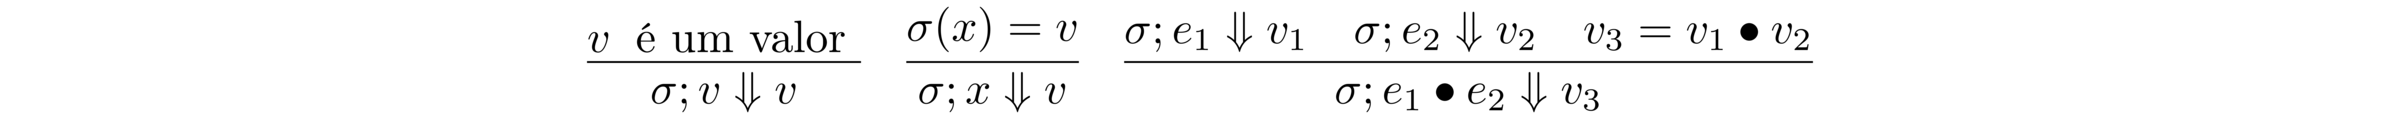
\includegraphics[width=.9\linewidth]{./imgs/image1.png}
\end{center}
\subsection*{Semântica de Imp}
\label{sec:orgdd936c0}

\begin{itemize}
\item Semântica big-step
\end{itemize}

\begin{center}
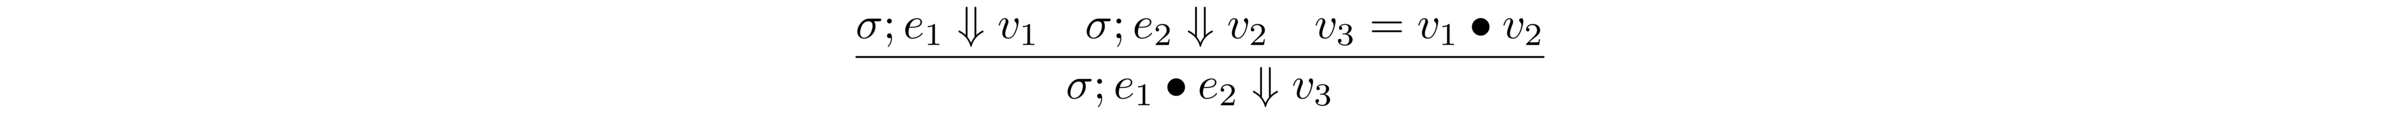
\includegraphics[width=.9\linewidth]{./imgs/image2.png}
\end{center}
\subsection*{Semântica de Imp}
\label{sec:org9ec28c0}

\begin{itemize}
\item Definição de uma mônada
\end{itemize}

\begin{verbatim}
type Env = Map (Var String) Value

type ExecM a = ExceptT String (StateT Env IO) a
\end{verbatim}
\subsection*{Semântica de Imp}
\label{sec:org04632d4}

\begin{itemize}
\item Operações sobre a mônada
\end{itemize}

\begin{verbatim}
insertEnv :: Var String -> Value -> ExecM ()
insertEnv v val = modify (insert v val)

removeEnv :: [Var String] -> ExecM ()
removeEnv vs = modify (\ env -> foldr delete env vs)
\end{verbatim}
\subsection*{Semântica de Imp}
\label{sec:org0f70320}

\begin{verbatim}
lookupEnv :: Var String -> ExecM Value
lookupEnv v
  = do
       val <- gets (lookup v)
       case val of
         Nothing -> throwError $ "Variable undefined:" ++ (unVar v)
         Just val' -> return val'
\end{verbatim}
\subsection*{Semântica de Imp}
\label{sec:org4d1357a}

\begin{itemize}
\item Definição de duas funções.
\begin{itemize}
\item Semântica de expressões
\item Semântica de comandos.
\end{itemize}
\end{itemize}
\subsection*{Semântica de Imp}
\label{sec:org71a8f5f}

\begin{itemize}
\item Semântica de expressões
\begin{itemize}
\item Valores
\end{itemize}
\end{itemize}

\begin{verbatim}
semanticsExpr :: Exp String -> ExecM Value
semanticsExpr (EValue v) = return v
\end{verbatim}
\subsection*{Semântica de Imp}
\label{sec:org7b81d6f}

\begin{itemize}
\item Semântica de expressões
\begin{itemize}
\item Variáveis
\end{itemize}
\end{itemize}

\begin{verbatim}
semanticsExpr (EVar v) = lookupEnv v
\end{verbatim}
\subsection*{Semântica de Imp}
\label{sec:org32e5f22}

\begin{itemize}
\item Semântica de expressões
\begin{itemize}
\item Operadores
\end{itemize}
\end{itemize}

\begin{verbatim}
(.+.) :: Value -> Value -> Value
(EInt n) .+. (EInt m) = EInt (n + m)
_ .+. _ = error "Impossible! Type Error"

semanticsExpr (e1 :+: e2)
  = do
       v1 <- semanticsExpr e1
       v2 <- semanticsExpr e2
       return $ v1 .+. v2
\end{verbatim}
\subsection*{Semântica de Imp}
\label{sec:orgd2afe0f}

\begin{itemize}
\item Semântica de comandos
\end{itemize}

\begin{verbatim}
semanticsStmt :: Stmt String -> ExecM [Var String]
semanticsStmt Skip = return []
semanticsStmt (Def ty v e)
  = do
      val <- maybe (return $ defaultValue ty) semanticsExpr e
      insertEnv v val
      return [v]
\end{verbatim}
\subsection*{Semântica de Imp}
\label{sec:orgfc66bd4}

\begin{itemize}
\item Semântica de comandos
\end{itemize}

\begin{verbatim}
semanticsStmt (v := e)
  = do
      val <- semanticsExpr e
      insertEnv v val
      return []
semanticsStmt (If e blk1 blk2)
  = do
      val <- semanticsExpr e
      if val == EBool True then semanticsBlock blk1
        else semanticsBlock blk2
      return []
\end{verbatim}
\subsection*{Semântica de Imp}
\label{sec:org093ac6b}

\begin{itemize}
\item Semântica de comandos
\end{itemize}

\begin{verbatim}
semanticsStmt (Print e)
  = do
      val <- semanticsExpr e
      liftIO (putStr (render (pprint val)))
      return []
semanticsStmt (SRead v)
  = do
       inp <- liftIO getLine
       case parse parserValue "" inp of
         Left _ -> throwError "invalid input!"
         Right val -> insertEnv v val >> return []
\end{verbatim}
\subsection*{Semântica de Imp}
\label{sec:orgb51369b}

\begin{itemize}
\item Semântica de comandos
\end{itemize}

\begin{verbatim}
semanticsStmt (While e blk)
  = do
      val <- semanticsExpr e
      if val == EBool True then do
        semanticsBlock blk
        semanticsStmt (While e blk)
      else return []
\end{verbatim}
\subsection*{Semântica de Imp}
\label{sec:orgb5a4dfe}

\begin{itemize}
\item Semântica de blocos
\end{itemize}

\begin{verbatim}
semanticsBlock :: Block String -> ExecM ()
semanticsBlock (Block blk)
  = do
      vs <- concat <$> mapM semanticsStmt blk
      removeEnv vs
\end{verbatim}
\section*{Concluindo}
\label{sec:orgc859b39}

\subsection*{Concluindo}
\label{sec:org5ff71b2}

\begin{itemize}
\item Apresentamos a semântica operacional da linguagem Imp.

\item Apresentamos como esta é a especificação de um interpretador desta linguagem.
\end{itemize}
\subsection*{Concluindo}
\label{sec:org805418b}

\begin{itemize}
\item Apresentamos a implementação do interpretador em Haskell.
\end{itemize}
\section*{Exercícios}
\label{sec:org97cf130}

\subsection*{Exercícios}
\label{sec:org0d195ce}

\begin{itemize}
\item O interpretador de Imp não provê suporte a valores de String.
Modifique a implementação de Imp de forma a permitir Strings e
também adicione a operação de concatenação de strings.
\end{itemize}
\end{document}
